\chapter{نتایج}
\section{معیارهای ارزیابی در یادگیری عمیق}

در این بخش، به بررسی معیارهای مختلفی که برای ارزیابی مدل‌های یادگیری عمیق استفاده می‌شوند، می‌پردازیم. این معیارها شامل \lr{Sensitivity}، \lr{Specificity}، \lr{Precision}، \lr{F1 Score}، \lr{Accuracy}، \lr{Intersection over Union (IoU)} و ضریب \lr{Dice} می‌باشد.

قبل از پرداختن به تعریف این معیارها، ابتدا به تعریف چهار مفهوم اساسی می‌پردازیم که در فرمول‌های ارزیابی به‌کار می‌روند:

\begin{itemize}
    \item \textbf{\lr{TP} \lr{(True Positives)}}: تعداد نمونه‌های مثبت که به‌درستی به‌عنوان مثبت دسته‌بندی شده‌اند.
    \item \textbf{\lr{FP} \lr{(False Positives)}}: تعداد نمونه‌های منفی که به اشتباه به‌عنوان مثبت دسته‌بندی شده‌اند.
    \item \textbf{\lr{TN} \lr{(True Negatives)}}: تعداد نمونه‌های منفی که به‌درستی به‌عنوان منفی دسته‌بندی شده‌اند.
    \item \textbf{\lr{FN} \lr{(False Negatives)}}: تعداد نمونه‌های مثبت که به اشتباه به‌عنوان منفی دسته‌بندی شده‌اند.
\end{itemize}

\subsection{\lr{Sensitivity}}

\lr{Sensitivity}، که با نام نرخ تشخیص صحیح نیز شناخته می‌شود، معیاری برای ارزیابی توانایی مدل در تشخیص صحیح نمونه‌های مثبت است. فرمول این معیار در \autoref{eq:sensitivity} مشخص شده است.

\begin{latin}
\begin{equation}
\label{eq:sensitivity}
\text{Sensitivity} = \frac{TP}{TP + FN}
\end{equation}
\end{latin}

\subsection{\lr{Specificity}}

\lr{Specificity}، معیاری است که نشان‌دهنده توانایی مدل در شناسایی صحیح نمونه‌های منفی است. فرمول این معیار در \autoref{eq:specificity} مشخص شده است.

\begin{latin}
\begin{equation}
\label{eq:specificity}
\text{Specificity} = \frac{TN}{TN + FP}
\end{equation}
\end{latin}

\subsection{\lr{Precision}}

\lr{Precision}، معیاری برای ارزیابی میزان درستی دسته‌بندی نمونه‌های مثبت است. به عبارت دیگر، \lr{Precision} نسبت نمونه‌های مثبت درست دسته‌بندی شده به تمام نمونه‌های پیش‌بینی‌شده به عنوان مثبت است. فرمول آن در \autoref{eq:precision} مشخص شده است.

\begin{latin}
\begin{equation}
\label{eq:precision}
\text{Precision} = \frac{TP}{TP + FP}
\end{equation}
\end{latin}

\subsection{\lr{F1 Score}}

\lr{F1 Score}، میانگین موزون \lr{Precision} و \lr{Sensitivity} است که تعادلی بین این دو معیار ایجاد می‌کند. این امتیاز به‌ویژه در مواردی که تعادل بین \lr{Precision} و \lr{Sensitivity} اهمیت دارد، مورد استفاده قرار می‌گیرد. فرمول \lr{F1 Score} در \autoref{eq:f1_score} مشخص شده است.

\begin{latin}
\begin{equation}
\label{eq:f1_score}
\text{F1 Score} = 2 \times \frac{\text{Precision} \times \text{Sensitivity}}{\text{Precision} + \text{Sensitivity}}
\end{equation}
\end{latin}

\subsection{\lr{Accuracy}}

\lr{Accuracy}، نسبت نمونه‌هایی است که به‌درستی دسته‌بندی شده‌اند به تمام نمونه‌ها. این معیار نشان‌دهنده عملکرد کلی مدل است و فرمول آن در \autoref{eq:accuracy} مشخص شده است.

\begin{latin}
\begin{equation}
\label{eq:accuracy}
\text{Accuracy} = \frac{TP + TN}{TP + TN + FP + FN}
\end{equation}
\end{latin}

\subsection{\lr{Intersection over Union (IoU)}}

\lr{Intersection over Union}، که به عنوان \lr{Jaccard Index} نیز شناخته می‌شود، معیاری است که برای ارزیابی همپوشانی بین دو مجموعه، به‌ویژه در مسائل بخش‌بندی تصویر، استفاده می‌شود. فرمول \lr{IoU} در \autoref{eq:iou} مشخص شده است.

\begin{latin}
\begin{equation}
\label{eq:iou}
\text{IoU} = \frac{|A \cap B|}{|A \cup B|} = \frac{TP}{TP + FP + FN}
\end{equation}
\end{latin}

\subsection{\lr{Dice Coefficient}}

ضریب \lr{Dice}، مشابه \lr{IoU} است اما وزن بیشتری به ناحیه اشتراک می‌دهد و در مسائل بخش‌بندی تصویر بسیار مورد استفاده قرار می‌گیرد. فرمول ضریب \lr{Dice} در \autoref{eq:dice} مشخص شده است.

\begin{latin}
\begin{equation}
\label{eq:dice}
\text{Dice Coefficient} = \frac{2 \times |A \cap B|}{|A| + |B|} = \frac{2 \times TP}{2 \times TP + FP + FN}
\end{equation}
\end{latin}

\section{نتایج طبقه‌بندی}

در این بخش، نتایج حاصل از مدل‌های طبقه‌بندی خونریزی داخل‌جمجمه‌ای در تصاویر سی‌تی‌اسکن، بررسی و تحلیل شده‌اند. تمرکز اصلی آموزش مدر طبقه‌بندی بر روی بهینه‌سازی فراپارامترها برای مدل
 \lr{ResNet50}
  بوده است، که بهبودهای قابل توجهی در عملکرد مدل به‌ویژه در معیار \lr{Sensitivity}
   به همراه داشته است.

\subsection{نتایج برش‌محور }
پس از آموزش مدل طبقه‌بندی برای تمام 
\lr{Fold}ها،
نمودار امتیاز
\lr{F1}
نسبت‌به آستانه‌های متفاوت رسم شد و در گام بعدی میانگین این نمودارها محاسبه شد. در انتها بهترین آستانه روی میانگین این نمودار‌ها محاسبه شده و در محاسبه معیارهای مربوط به زیرمجموعه ارزیابی استفاده شده است.
 \autoref{tab:slice_level_results}
  نتایج به‌دست‌آمده از آموزش مدل‌های \lr{ResNet50} و سازوکار شورا برای طبقه‌بندی برش‌محور نشان می‌دهد. همانطور که در جدول مشاهده می‌شود، بهترین نتایج در
 \lr{Fold 0}
  به‌دست آمده است که امتیاز 
  \lr{F1}
   برابر با
  $0.62$
 را نشان می‌دهد. این نشان‌دهنده این است که توزیع داده‌ها در مجموعه‌های آموزشی و اعتبارسنجی این 
 \lr{Fold}
  بیشتر شبیه به مجموعه آزمون است. در مقابل، 
  \lr{Fold 4}
   کمترین نتایج را به‌دست آورده، در حالی که نتایج مراحل دیگر با هم بیشتر هم‌خوانی دارند.


% Please add the following required packages to your document preamble:
% \usepackage{graphicx}
\begin{table}[h]
\centering
\caption{نتایج برش‌محور مدل \lr{ResNet50}
برای آستانه تصمیم‌گیری
$0.27$}
\label{tab:slice_level_results}
\resizebox{\textwidth}{!}{%
\begin{tabular}{llllll}
\textbf{مدل}           & \textbf{\lr{Sensitivity}} & \textbf{\lr{Specificity}} & \textbf{\lr{Precision}} & \textbf{\lr{F1}}   & \textbf{\lr{Accuracy}} \\ \hline
\lr{ResNet50 Fold 0}        & $0.78$            & $0.93$             & $0.51$         & $0.62$ & $0.91$    \\
\lr{ResNet50 Fold 1}        & $0.68$            & $0.90$             & $0.38$         & $0.49$ & $0.88$    \\
\lr{ResNet50 Fold 2}        & $0.60$            & $0.89$             & $0.33$         & $0.42$ & $0.86$    \\
\lr{ResNet50 Fold 3}        & $0.86$            & $0.89$             & $0.41$         & $0.55$ & $0.89$    \\
\lr{ResNet50 Fold 4}        & $0.32$            & $\mathbf{0.96}$             & $0.42$         & $0.36$ & $0.90$    \\ \hline
\lr{Neethi et al.} {[}\lr{19}{]} & $0.76$            & $-$                & $\mathbf{0.69}$         & $\mathbf{0.67}$ & $0.54$    \\
\lr{someone}                & $1$               & $2$                & $3$            & $4$    & $5$       \\ \hline
\lr{ResNet50 Voting}        & $\mathbf{0.94}$            & $0.91$             & $0.49$         & $0.64$ & $\mathbf{0.91}$   
\end{tabular}%
}
\end{table}



همانطور که در 
\ref{fig:ch3-f1-vs-th-cls}
 مشاهده می‌شود، با استفاده از سازوکار شورایی، امتیاز \lr{F1} بهبود قابل توجهی پیدا کرده است که نشان‌دهنده بهبود عملکرد مدل طبقه‌بندی با استفاده از سازوکار شورایی است.
 \lr{Sensitivity}
  مدل به صورت برش‌محور 
 $0.94$ 
 بوده که یک دستاورد قابل توجه در مقایسه با سایر مطالعات است خصوصا در زمینه استفاده‌های پزشکی. نکته‌ای که باید به آن توجه کرد این است که مقادیر گزارش‌شده برای
 \lr{Fold}های 
 متفاوت،‌ به‌ازای آستانه‌های متفاوت می‌توانند مقادیر بهتری داشته باشند اما اعداد گزارش شده در بهترین آستانه برای میانگین نمودارها می‌باشد.
\autoref{fig:ch3-metrics-cls}
نمودارهای
			\lr{Sensivity, Precision} و امتیاز\lr{F1}
			به ازای آستانه‌های متفاوت را نشان می‌دهد و 
\autoref{fig:ch3-metrics and pr cls}
نمودار منحنی 
\lr{Precision-Sensitivity}
را نشان می‌دهد.
\autoref{fig:ch3-s-cm}
ماتریس آشفتگی مدل‌ها را نشان می‌دهد،‌ همانطور که مشخص است مدلی که از سازوکار شورایی استفاده می‌کند به صورت قابل توجهی عملکرد بهتری پیدا می‌کند.
\begin{figure}[h]
\centering
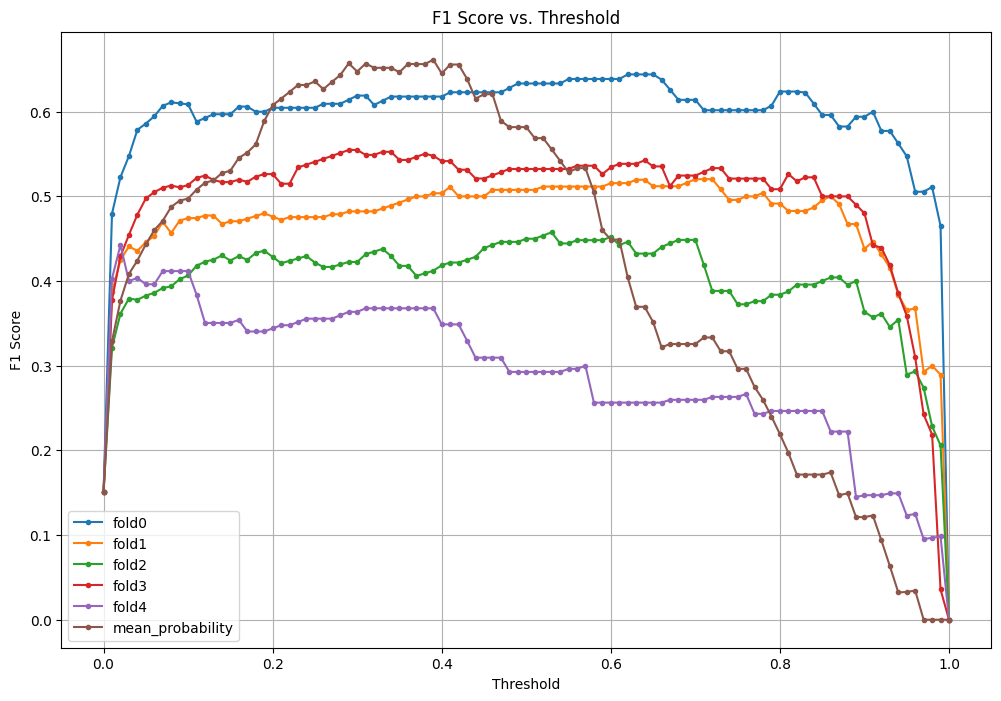
\includegraphics[width=1.0\linewidth]{Images/Chapter3/f1-vs-th-cls}
\caption{نمودار امتیاز \lr{F1} نسبت به آستانه برای \lr{Fold}ها و میانگین آنها}
\label{fig:ch3-f1-vs-th-cls}

\end{figure}


\begin{figure}[h!]
		\centering % <-- added
		\begin{subfigure}{0.45\textwidth}
			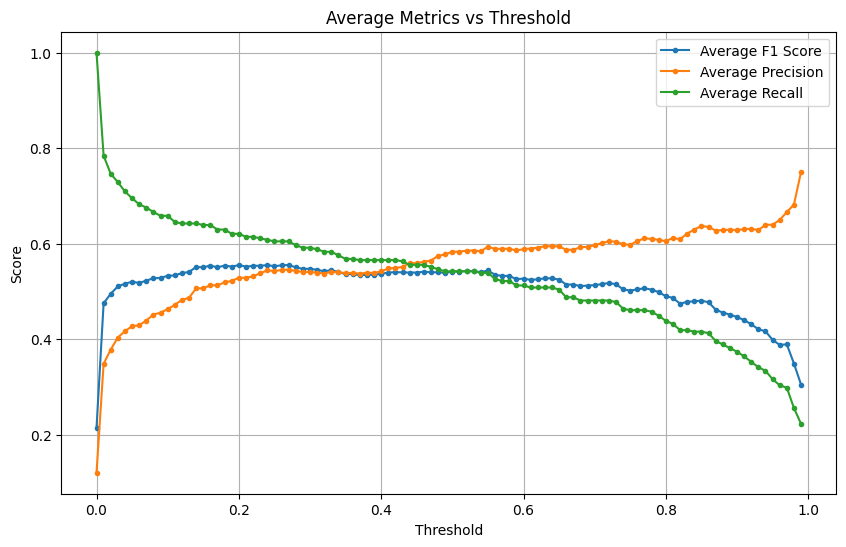
\includegraphics[width=\linewidth]{Images/Chapter3/metrics-cls.png}
			\caption{}
			
			\label{fig:ch3-metrics-cls}
		\end{subfigure}\hfil % <-- 
		\begin{subfigure}{0.45\textwidth}
			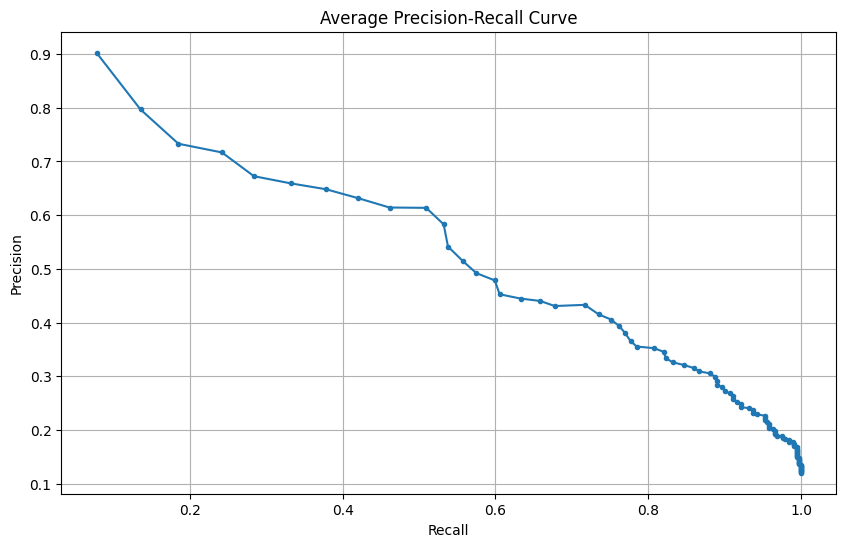
\includegraphics[width=\linewidth]{Images/Chapter3/pr-cls.png}
			\caption{}
			\label{fig:ch3-pr-cls}
		\end{subfigure}\hfil % <-- added
		\caption{نمودارهای سازوکار شورایی روی مجموعه‌داده ارزیابی}
		\label{fig:ch3-metrics and pr cls}
\end{figure}


\begin{figure}[h]
\centering
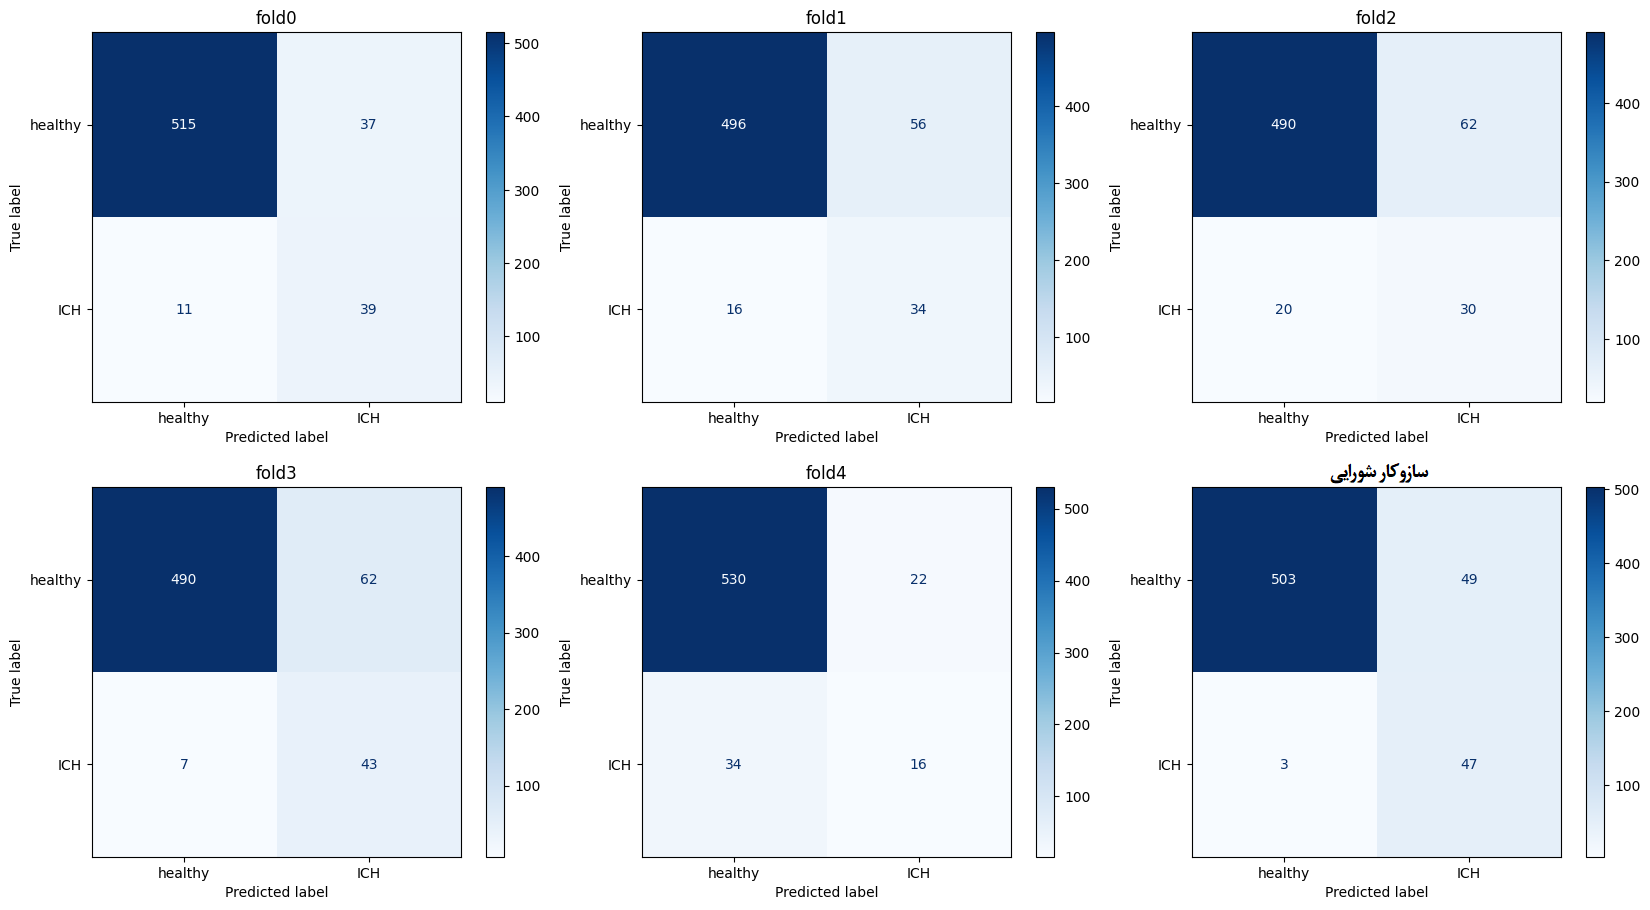
\includegraphics[width=1.0\linewidth]{Images/Chapter3/s-cm}
\caption{ماتریس آشفتگی نتایج برش‌محور}
\label{fig:ch3-s-cm}
\end{figure}







\subsection{نتایج بیمارمحور}

طبقه‌بندی بیمارمحور خونریزی درون‌جمجمه‌ای بر اساس پیش‌بینی‌های برش‌محور انجام شده است. یک بیمار در صورتی دارای خونریزی درون‌جمجمه‌ای در نظر گرفته می‌شود اگر حداقل یک برش از سی‌تی‌اسکن او دارای علائم خونریزی شناسایی شود. نتایج به‌دست‌آمده نشان می‌دهند که مدل 
\lr{ResNet50}
 در بررسی بیمارمحور سی‌تی‌اسکن‌ها، با استفاده از روش شورایی، به 
 \lr{Sensitivity}
  برابر با
   $1.00$، 
   \lr{Specificity}
برابر با
     $0.80$، \lr{Precision}
      برابر با
       $0.75$،
        امتیاز
         \lr{F1}
          برابر با
           $0.86$
            و 
            \lr{Accuracy}
             برابر با
              $0.88$ 
              دست یافته است که از تمامی معیارهای گزارش شده در سایر مطالعات، نتیجه بهتری کسب کرده است.
جدول \ref{tab:patient_level_results} نتایج بیمارمحور مدل \lr{ResNet50} را برای هر مرحله آموزشی نشان می‌دهد.
\autoref{fig:ch3-p-cm}
ماتریس آشفتگی بیمارمحور را نشان می‌دهد که از 16 بیمار در مجموعه ارزیابی قرار داشته‌اند که همه 6 بیمار دارای خونریزی درست تشخیص داده شده‌اند.

% Please add the following required packages to your document preamble:
% \usepackage{graphicx}
\begin{table}[]
\centering
\caption{نتایج بیمارمحور مدل \lr{ResNet50}
برای آستانه تصمیم‌گیری 
$0.27$}
\label{tab:patient_level_results}
\resizebox{\textwidth}{!}{%
\begin{tabular}{llllll}
\textbf{مدل}          & \textbf{\lr{Sensitivity}} & \textbf{\lr{Specificity}} & \textbf{\lr{Precision}} & \textbf{\lr{F1}}            & \textbf{\lr{Accuracy}}      \\ \hline
\lr{ResNet50 Fold 1}       & $1.00$                 & $0.60$                 & $0.60$               & $0.75$          & $0.75$          \\
\lr{ResNet50 Fold 2}       & $1.00$                 & $0.60$                 & $0.60$               & $0.75$          & $0.75$          \\
\lr{ResNet50 Fold 3}       & $1.00$                 & $0.60$                 & $0.60$               & $0.75$          & $0.75$          \\
\lr{ResNet50 Fold 4}       & $0.83$                 & $0.80$                 & $0.71$               & $0.77$          & $0.81$          \\ \hline
\lr{Kyung et al.} {[}\lr{14}{]} & $0.97$                 & $0.74$                 & $-$                  & $0.84$          & $-$             \\ \hline
\lr{ResNet50 Voting}       & $\mathbf{1.00}$        & $\mathbf{0.80}$        & $\mathbf{0.75}$      & $\mathbf{0.86}$ & $\mathbf{0.88}$
\end{tabular}%
}
\end{table}
\begin{figure}[h]
\centering
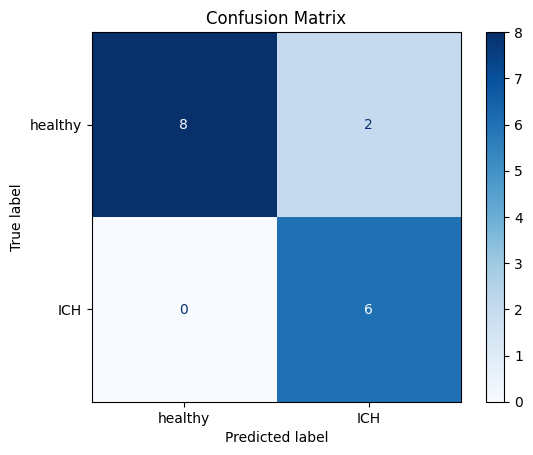
\includegraphics[width=1.0\linewidth]{Images/Chapter3/p-cm}
\caption{ماتریس آشفتگیب یمارمحور سازوکار شورایی}
\label{fig:ch3-p-cm}
\end{figure}


\subsection{تحلیل بیشتر نتایج}

در این بخش، نتایج مرتبط با تفسیرپذیری مدل \lr{ResNet50} از طریق تکنیک‌های \lr{Grad-CAM} و \lr{t-SNE} تحلیل و بررسی می‌شوند.

\subsubsection{تحلیل \lr{Grad-CAM}}

تکنیک 
\lr{Gradient-weighted Class Activation Mapping}
(\lr{Grad-CAM})
 به عنوان یک ابزار قدرتمند برای تفسیر مدل‌های شبکه عصبی عمیق استفاده می‌شود. این تکنیک به ما اجازه می‌دهد تا ببینیم کدام بخش‌های تصویر ورودی، بیشتر در تصمیم‌گیری مدل تأثیر داشته‌اند. در این پروژه، از روش
 \lr{Grad-CAM}
  برای افزایش تفسیرپذیری مدل‌های طبقه‌بندی به کمک ایجاد تصویر استفاده شده است که نواحی مهم برش‌های سی‌تی‌اسکن که منجر به تشخیص خونریزی توسط مدل شده‌اند را مشخص می‌‌کند.  
  \autoref{fig:ch3-gradcam} 
  نمونه‌ای از این نقشه‌های حرارتی را نشان می‌دهد که به وضوح مشخص می‌کند که مدل چگونه نواحی مختلف تصویر را برای تشخیص \lr{ICH} مورد ارزیابی قرار داده است.
\begin{figure}[h]
\centering
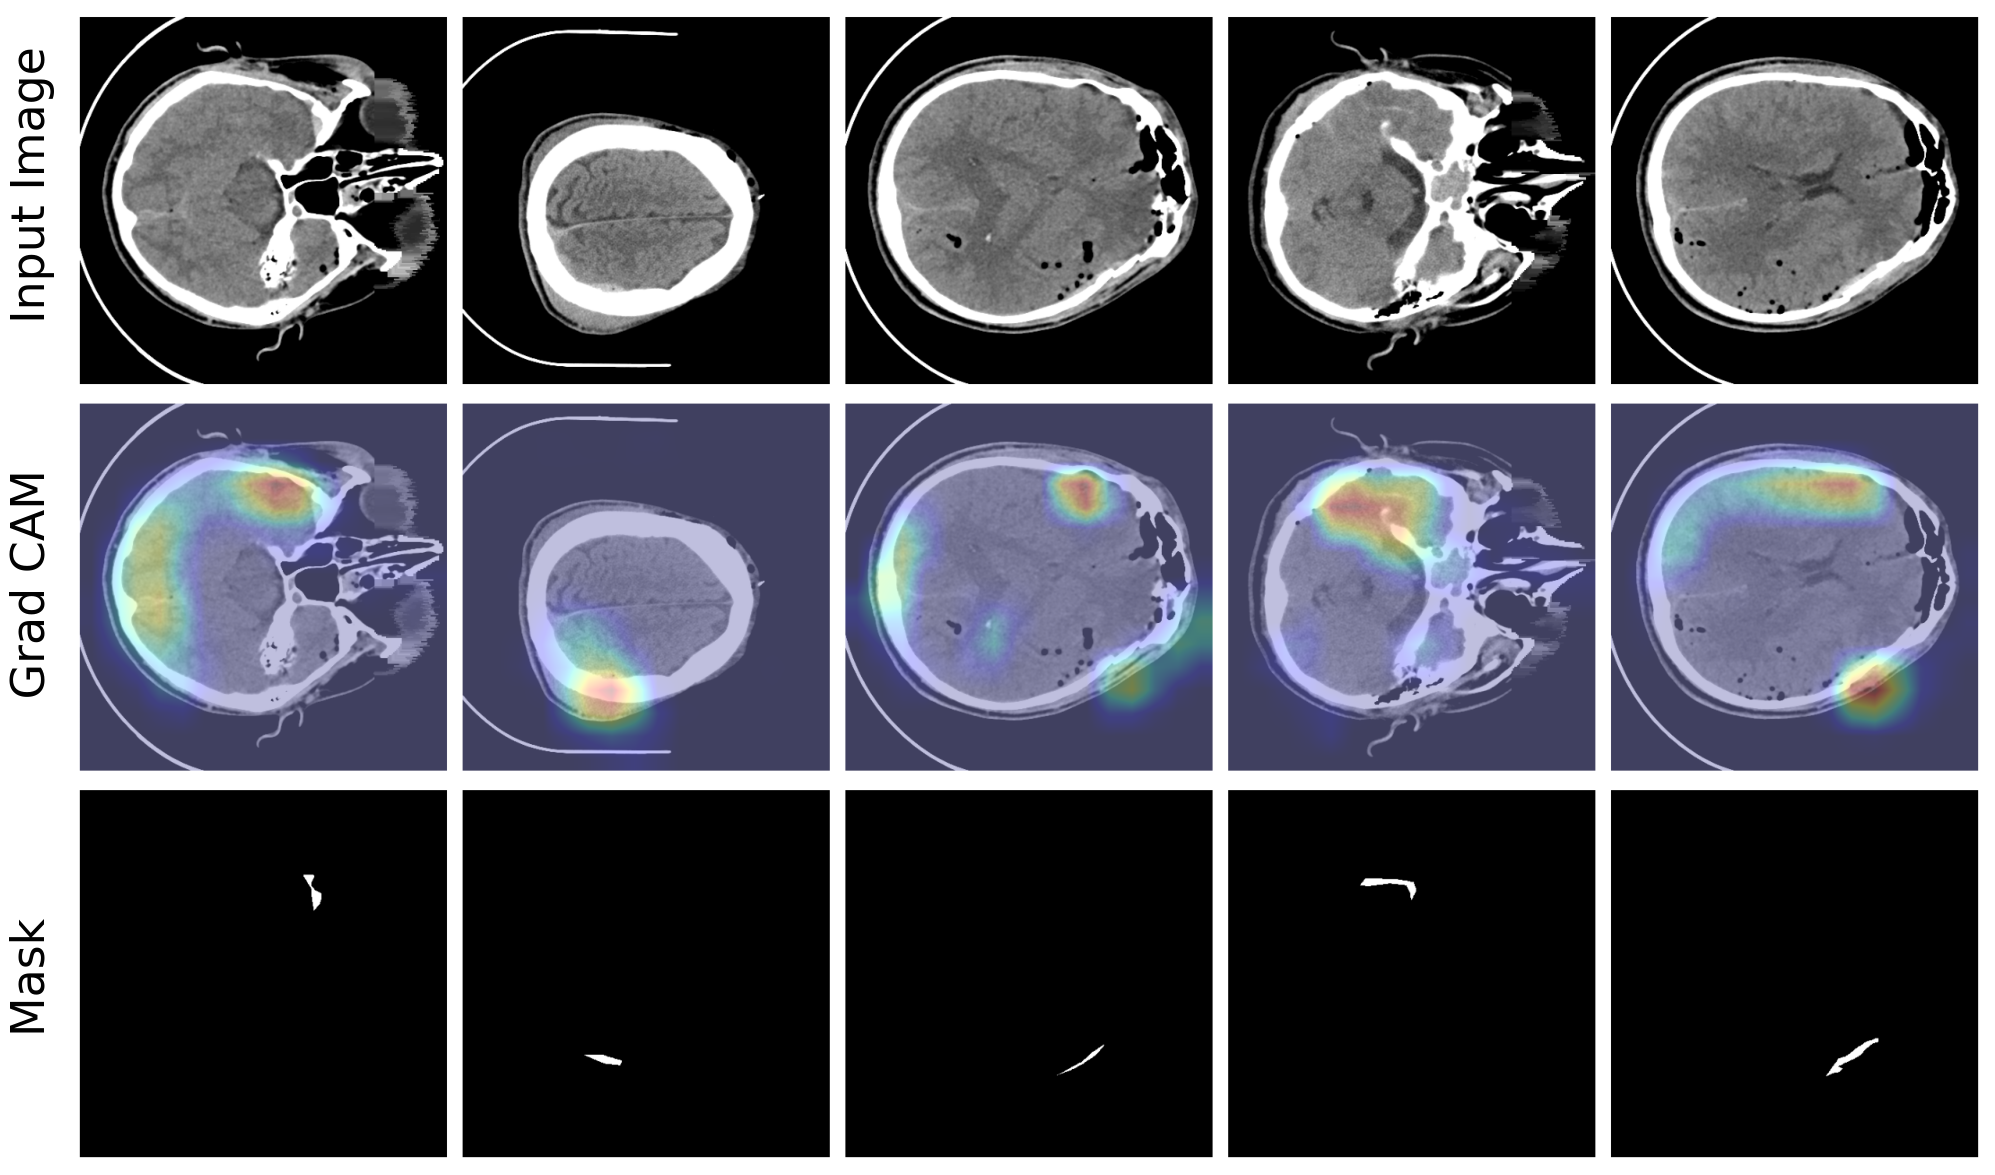
\includegraphics[width=1.0\linewidth]{Images/Chapter3/GradCam}
\caption{چند نمونه از تصاویر تولید شده توسط  \lr{Grad-CAM}}
\label{fig:ch3-gradcam}
\end{figure}

\subsubsection{تحلیل \lr{t-SNE}}

روش
 \lr{t-Distributed Stochastic Neighbor Embedding} (\lr{t-SNE})
  یک روش برای کاهش ابعاد و تجسم داده‌های با ابعاد بالا است. در این پژوهش، از
   \lr{t-SNE}
    برای تجسم توزیع ویژگی‌های استخراج‌شده از مدل \lr{ResNet50} 
    استفاده شده است تا نشان داده شود که آموزش مدل، باعث تولید ویژگی‌هایی شده است که تفکیک‌پذیری برش‌های سالم را از ناسالم زیاد کرده است. 
     \autoref{fig:ch3-tsne}
 نشان‌دهنده توزیع ویژگی‌های استخراجی با روش 
 \lr{t-SNE}
  از تصاویر سی‌تی‌اسکن در فضای دو‌بعدی است که 
  \autoref{fig:ch3-tsne-before}
  پراکندگی ویژگی‌ها از مدل طبقه‌بندی قبل از آموزش آن است و 
    \autoref{fig:ch3-tsne-after}
    بعد از آموزش مدل طبقه‌بندی است. 
      \autoref{fig:ch3-tsne-before}
  به‌وضوح نشان می‌دهد چگونه مدل قادر است تفکیک‌پذیری خطی را برای برش‌های حاوی خونریزی درون‌جمجمه‌ای ایجاد کند. این استخراج ویژگی کمک می‌کند تا دیدگاه بهتری نسبت به نحوه عملکرد مدل در سطح ویژگی‌ها داشته باشیم و نقاط ضعف و قوت آن را بهتر درک کنیم. 
        \autoref{fig:ch3-tsne-other}
نمودار 
\lr{t-SNE}
حاصل از مدل طبقه‌بندی 
\lr{Ganeshkumar}\cite{Ganeshkumar2022Identification}
و همکاران است که نشان می‌دهد مدل بدست‌آمده در پژوهش آنها، امکان تفکیک‌پذیری خطی را برای برش‌ها ایجاد نکرده است.

\begin{figure}[h!]
		\centering % <-- added
		\begin{subfigure}{0.33\textwidth}
			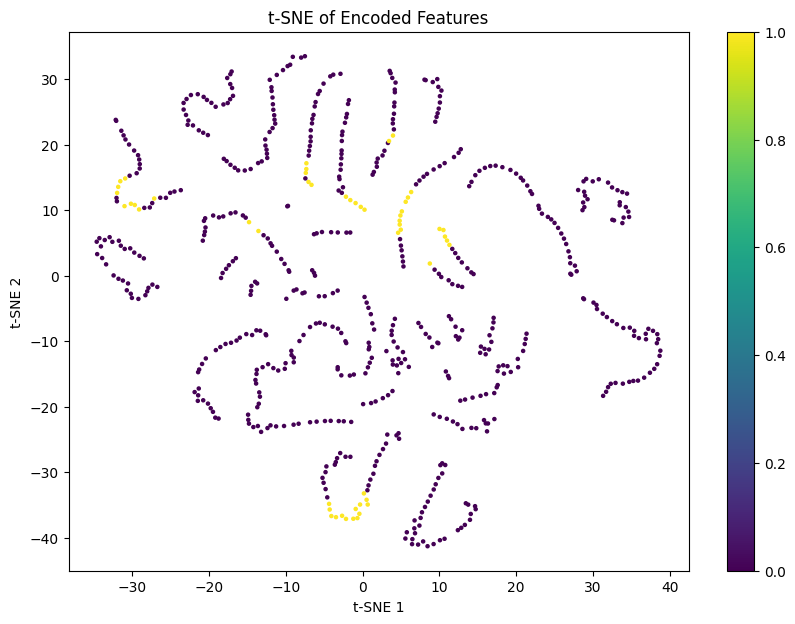
\includegraphics[width=\linewidth]{Images/Chapter3/tsne_vanilla.png}
			\caption{قبل از آموزش}
			\label{fig:ch3-tsne-before}
		\end{subfigure}\hfil % <-- 
		\begin{subfigure}{0.33\textwidth}
			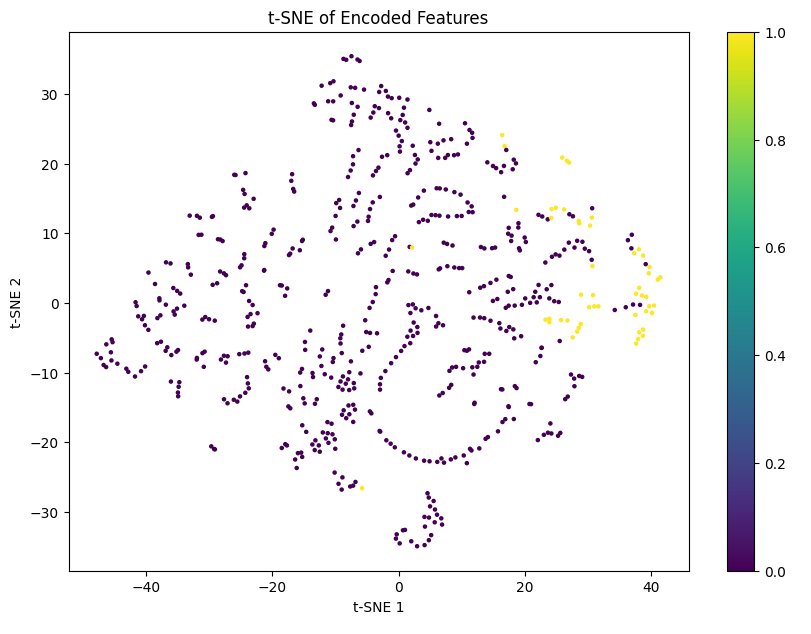
\includegraphics[width=\linewidth]{Images/Chapter3/tsne.png}
			\caption{بعد از آموزش}
			\label{fig:ch3-tsne-after}
		\end{subfigure}\hfil % <-- added
        \begin{subfigure}{0.33\textwidth}
			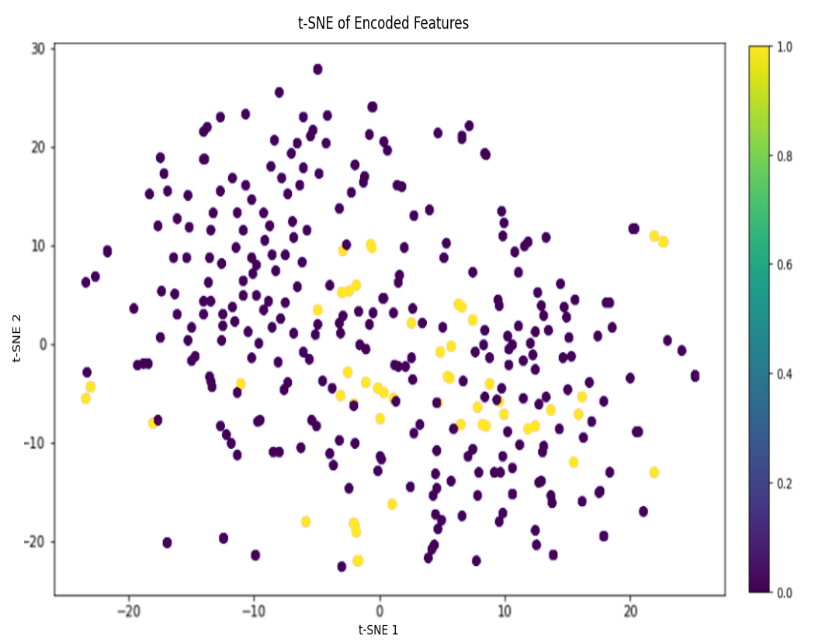
\includegraphics[width=\linewidth]{Images/Chapter3/tsne-other.png}
			\caption{مدل  
			\lr{Ganeshkumar} 
			\cite{Ganeshkumar2022Identification}}
			\label{fig:ch3-tsne-other}
        \end{subfigure}
		\caption{نمودارهای 
		\lr{t-SNE}
		و مقایسه آنها با یکدیگر}
		\label{fig:ch3-tsne}
\end{figure}